L'algorithme de couverture est une am\'elioration de  celui de Lehot \cite{decompositionEnCliquesParArcs}.
En effet, l'algorithme de Lehot se subdivise en deux parties : 
La premi\`ere partie consiste \`a nommer des sommets appartenant \'a une m\^eme clique et la seconde partie \`a comparer, s'il existe, le line graphe propos\'e avec celui du graphe racine. 
Concernant l'identification, il distingue 5 categories de sommets:
\begin{itemize}
\item les sommets ``well-defined" : des sommets du graphe racine $G$ dont leur clique correspondante dans $L(G)$ a \'et\'e trouv\'ee et identifi\'ee.
\item les sommets ``half-named" : des sommets de $L(G)$ dont un sommet de leur ar\^ete dans $G$ a d\'ej\`a \'et\'e ``well-defined".
\item les sommets ``fully-named" : des ar\^etes de $G$ dont leurs sommets dans $L(G)$ sont "well-defined".
\item les sommets ``basics" : sommets adjacents dans $L(G)$. Not\'e $2-3$, chaque chiffre est un sommet dans $G$.
\item les sommets ``cross" : sommets adjacents aux sommets ``basics" appartenant \`a deux cliques.
\end{itemize}
Le but de cet algorithme est d'identifier les sommets ``cross" parmi les sommets adjacents d'un sommet de $L(G)$ \`a partir des trois cas \cite{decompositionEnCliquesParArcs}. \newline
L'algorithme d\'ebute par la s\'election de deux sommets ``basics" $1-2, 2-3$ et de leur ensemble d'adjacents $X$.
Si $|X| = \emptyset$ alors tous les sommets des cliques sont identifi\'es en ``half-named".
Si $|X| = 1$ alors il existe un sommet $x$ adjacent aux deux sommets ``basics" ($1-2,2-3$) tel que $(x,1-2,2-3)$ forme un triangle ``odd" si $x=2-4$ ou un triangle ``even" si $x=1-3$. Le sommet $x$ devient {\em cross} et est identifi\'e en ``fully named". Les autres sommets $1-2,2-3$ sont identifi\'es en ``half-named".
Dans le cas o\`u  $|X = \{x,y\}|=2$, si $x$ et $y$ sont adjacents alors il n'existe pas de sommets ``cross" sinon ils forment deux triangles avec $1-2,2-3$. Un de ces triangles est ``odd" implique que $x=2-4$ , $y=1-3$ et $y$ est identifi\'e en sommet ``cross".
Enfin pour $|X =\{ a,b,...\}| \ge 3$, si $a$ et $b$ sont adjacents, $b$ est d\'eclar\'e sommet ``cross" sinon c'est le sommet $a$ qui le devient.
La derni\`ere \'etape s\'electionne al\'eatoirement un sommet $u$ ``half-named". Ce sommet est adjacent \`a un sommet $v$ ``fully-named". Si ce sommet $v$ n'est pas d\'ej\`a couvert par une clique, alors il existe un sommet $z$ ``fully-named" qui appartient d\'ej\`a \`a une clique et qui est d\'eclar\'e sommet ``cross" de ces deux pr\'ec\'edents sommets $u$ et $v$. Nous trouvons ces sommets $u$ et $v$ gr\^ace \`a une pile o\`u $u$ et $v$ sont en t\^ete et nous les nommons avec le num\'ero de la clique. 
\`A la fin de cette \'etape, tous les sommets sont nomm\'es ``fully-named" et nous identifions les sommets ``fully-named" adjacents par un nouveau num\'ero de clique.
\newline
Nous comparons le line-graphe propos\'e $H$ et le line-graphe $L(G)$ de $G$, ar\^etes par ar\^etes, et s'il existe une ar\^ete de $H$ n'ayant pas de correspondance dans $L(G)$ alors $L(G)$ n'est pas un line-graphe et l'algorithme ne retourne pas de r\'esultats c'est-\`a-dire aucunes cliques d\'ecouvertes lors du traitement des sommets.
Cet algorithme s'ex\'ecute en $O(N)+E$ avec $N$  le nombre d'ar\^etes dans $G$ et $E$ le nombre d'ar\^etes dans $L(G)$ car le processus d'identification des ar\^etes est en $O(N)$ et la comparaison entre graphes en $E$ \'etapes.
\newline

Notre algorithme de couverture  couvrira autant que possible des sommets du graphe de corr\'elation  $G_M$ par une ou deux cliques et si $G_M$ ne contient aucune erreur de corr\'elation alors il retourne sa line-couverture. Dans le cas contraire, les sommets couverts par plus de deux cliques sont sauvegard\'es dans l'ensemble des sommets \`a corriger $sommets\_1$ et notre algorithme retourne les cliques d\'ecouvertes et l'ensemble $sommets\_1$.

\subsubsection{Description de l'algorithme de couverture}
Soit le graphe de corr\'elation $G_M = (V,E)$.
Consid\'erons $\cal C$ un ensemble de cliques d\'ecouvertes de $G_M$ initialement vide et chaque sommet $v \in V$ a un \'etat  $Cliq(v)$ initialis\'e \`a $0$.
\newline
Chaque sommet $v$ a cinq \'etats possibles:
\begin{itemize}
	\item $0$ : il n'est couvert par aucune clique. Il correspond aussi \`a l'\'etat initial des sommets. C'est un sommet ``basic''.
	\item $1$ : le sommet $v$ est couvert par une clique ou deux cliques. Dans le cas o\`u il est couvert par deux cliques, l'intersection de ces cliques donne le sommet $v$. Ce sommet est identifi\'e par ``fully-named".
	\item $2$ : le sommet est couvert par une clique et peut \^etre couvert par une seconde clique. C'est un sommet ``well-named"
	\item $3$ : le sommet $v$ est un sommet ambigu. C'est un sommet ``cross''.
	\item $-1$ :  le sommet $v$ est couvert par plus de deux cliques. Il est contenu dans l'ensemble $sommets\_1$ et doit \^etre corrig\'e par l'algorithme de correction.
\end{itemize}
Nous choisissons un sommet $v$ de degr\'e minimum tel qu'il n'appartienne \`a aucune clique ou qu'il soit un sommet ambigu. 
S'il existe une partition coh\'erente de ce sommet et de son voisinage $\{v\} \cup \Gamma_{G_C}(v)$ en deux cliques $C_1, C_2$, alors ces deux cliques sont contenues dans la line-couverture $\cal C$. Les sommets $v$ et $u$ (avec $u \neq v$), appartenant \`a $C_1$ ou $C_2$, ont leurs \'etats modifi\'es de la mani\`ere suivante :
\begin{itemize}
\item $Cliq(v) = 1$ si son \'etat pr\'ec\'edent est \'egal \`a $0$ et la clique $C_2$ est vide. 
\item $Cliq(v) = 3$ si son \'etat pr\'ec\'edent est \'egal \`a $0$ et la clique $C_2$ est non vide. 
\item $Cliq(v) = 2$ si son \'etat pr\'ec\'edent est diff\'erent de $0$.
\item $Cliq(u) = 1$ si son \'etat pr\'ec\'edent est \'egal \`a $0$ et l'ensemble des ar\^etes incidentes \`a $u$ est vide.
\item $Cliq(u) = 2$ si son \'etat pr\'ec\'edent est \'egal \`a $3$ et l'ensemble des ar\^etes incidentes \`a $u$ est vide.
\item $Cliq(u) = 3$ si son \'etat pr\'ec\'edent est \'egal \`a $0$ et l'ensemble des ar\^etes incidentes \`a $u$ est non vide.
\item $Cliq(u) = -1$ si son \'etat pr\'ec\'edent est \'egal \`a $3$ et l'ensemble des ar\^etes incidentes \`a $u$ est non vide.
\end{itemize} 
Dans le cas ou il n'existe aucune partition coh\'erente au sommet $v$, son \'etat est \`a $Cliq(v)=-1$.

\begin{algorithm}[!ht]
\caption{couverture\_cliques}
\noindent DEBUT\\
\noindent 1. {\bf Si} $G_M$ est isomorphe \`a un graphe double (voir figure \ref{graphe2Couverture} ), {\bf alors} le traiter avec Verif\_correl$(^1)$ \\
~~\indent {\bf Sinon} \\
~2. \indent {\bf Tant que} il existe un sommet $u$ t.q $Cliq(u) \in \{0,3\}$\\ 
       	\indent~~~~~~{\bf Faire}\\
~3.	       	\indent~~~~~~~~choisir $u$ de degr\'e minimum\\
~4.       	\indent~~~~~~~~{\bf Si} $\{u\} \cup \Gamma_{G_M}(u)$ peut \^etre couvert par deux cliques $C_1$ et $C_2$ coh\'erentes,\\
		\indent~~~~~~~~~~~~~~$C_1$ maximale et $C_2 = \emptyset$ si $Cliq(u)=3$ $(^2)$\\
	       	\indent~~~~~~~~~~~~{\bf alors}\\
~5.	       	\indent~~~~~~~~~~~~~~{\bf Si } $Cliq(u) = 0$ et $C_2\neq \emptyset$ {\bf Alors} $Cliq = 3$ \\
~6.		\indent~~~~~~~~~~~~~~{\bf Sinon Si} $Cliq = 0$ et $C_2 =  \emptyset$ {\bf Alors} $Cliq(u) = 1$\\
~7.		\indent~~~~~~~~~~~~~~~~~~~~~~~{\bf Sinon} $Cliq(u) = 2$ 	\\
~8.		\indent~~~~~~~~~~~~~~~~~~~~~~~{\bf FinSi}\\      	
~9.		\indent~~~~~~~~~~~~~~{\bf FinSi}\\
~10.		\indent ~~~~~~~~~~~~~$\epsilon_u = E(G_M[C_1]) \cup E(G_M[C_2])$\\
~11.		\indent ~~~~~~~~~~~~~{\bf Pour tout} $w \in \Gamma_{G_M}(u)$ {\bf Faire} \\
~12.		\indent~~~~~~~~~~~~~~~~$\alpha(w) = card\{[w,x] \in E - \epsilon_u\}$\\
~13.		\indent~~~~~~~~~~~~~~~~{\bf Si} $\alpha_w > 0$ {\bf Alors}\\
~14.		\indent~~~~~~~~~~~~~~~~~~{\bf Si} $Cliq(w) = 0$ {\bf Alors} $Cliq(w) =3$\\
~15.		\indent~~~~~~~~~~~~~~~~~~{\bf Sinon Si} $Cliq(w) = 3$ {\bf Alors} $Cliq(w) =-1$\\
~16.		\indent~~~~~~~~~~~~~~~~~~{\bf FinSi} \\
~17.		\indent~~~~~~~~~~~~~~~~{\bf Sinon Si} $Cliq(w) = 0$ {\bf Alors} $Cliq(w) =1$\\
~18. 	\indent~~~~~~~~~~~~~~~~~~~~~~~~~{\bf Sinon Si} $Cliq(w) = 3$ {\bf Alors} $Cliq(w) = 2$ \\
~19. 	\indent~~~~~~~~~~~~~~~~~~~~~~~~~{\bf FinSi} \\
~20.		\indent ~~~~~~~~~~~~~{\bf FinPourTout}\\
~21.		\indent ~~~~~~~~~~~~~$E = E - \epsilon_u$\\
~22.		\indent            ~~~~~~~{\bf Sinon} $Cliq(u) = -1$\\
	       	\indent~~~~~~~~~~~~{\bf FinSi}\\
%       	\indent~~~~~~
~23. \indent {\bf FinTant que}\\
~24. \noindent {\bf Fin Si}\\
\noindent FIN\\
\end{algorithm}

$^1$ : chaque graphe de la figure \ref{graphe2Couverture} admet deux line-couvertures, souvent isomorphes, mais (au plus) une seule de ces line-couvertures correspond au DAG du r\'eseau \'electrique sous-jacent. Dans ce cas, on utilise les mesures de correlation de la matrice de mesures $\mu_C$ afin de d\'eterminer pla plus probable entre les deux.
\newline

 $^2$ :  le sommet $u$ choisi (s'il existe) ne sera pas prioritairement un sommet tel que $Cliq(u) = 0$ et $u$ est un point d'ambiguit\'e. Si lors d'une \'etape, seul un tel choix est possible et qu'il n'y a aucun sommet $u$ tel que $Cliq(u) = -1$, c'est que chaque sommet du graphe initial $G_M$ est un point d'ambiguit\'e.
 Dans ce cas, $G_M$ est une union de composantes connexes isomorphes \`a un des graphes de la figure  \ref{graphe2Couverture}.
Dans ce cas, n'importe quel choix conduit \`a une d\'ecomposition correcte.
Dans tous les autres cas de sommet choisi $u$, le lemme \ref{lemmaCoherente} montre que le choix de d\'ecomposition est unique si $G_M$ est un line graphe.
\newline

La partition coh\'erente se d\'etermine au moyen des mesures physiques selon la loi de conservation des noeuds \cite{loiDeConservation}. 
En effet, tous les sommets d'une clique dans un line-graphe sont des ar\^etes qui concourent un sommet du r\'eseau \'electrique. 
Par les lois d'\'electricit\'es, la diff\'erence entre les flots entrant et sortant dans ce sommet correspond aux pertes par effets joules $EJ$. 
Ainsi une clique s'obtient si cette diff\'erence est inf\'erieure aux pertes joules.
Dans notre algorithme de couverture, nous supposons que la partition coh\'erente propos\'ee est toujours exacte. Cela signifie que nous connaissons la valeur des pertes par effets joules dans le r\'eseau \'electrique. Dans le cas o\`u ce param\`etre est inconnu, quel est la valeur minimum de ces pertes not\'ee $\epsilon$ \`a partir de laquelle la partition est toujours exacte?
En d'autres termes, quel est la valeur $\epsilon$ pour laquelle la d\'ecision de l'ORACLE est un {\em vrai positif}, L'ORACLE \'etant la fonction retournant les partitions coh\'erentes. 
La d\'ecision de l'ORACLE est une valeur bool\'eenne.

\subsubsection{Impact des pertes par effets joules}
%epsilon est le taux min des pertes par effets joules pour lequel l'oracle ne comet pas d'erreurs.
% EJ ce sont les pertes par effet joules dans le reseau.
Nous consid\'erons que le r\'eseau \'electrique modelis\'e par un DAG $G$ est connu et que sa matrice de corr\'elation est correcte. 
Dans le but d'\'etudier le taux minimum des pertes par effets joules not\'ee $\epsilon$ dans le r\'eseau afin que la partition coh\'erente propos\'ee par  l'ORACLE soit toujours correcte, 
nous cherchons les ensembles arcs entrants $S_1$ et sortants $S_2$ d'un sommet tel que $ORACLE(S_1, S_2) = 1$.
Nous d\'efinissons la similarit\'e comme \'etant le pourcentage d'arcs bien pr\'edits par rapport aux arcs de $G$. 
Nous r\'ealisons deux exp\'eriences: 
\begin{itemize}
\item La premi\`ere exp\'erience consiste \`a g\'en\'erer des mesures de flots de divers graphes en faisant varier, de $0$ \`a $1$ par pas de $0.125$, les pertes par effets joules $EJ$ tout en fixant la variable $\epsilon$. Nous ex\'ecutons l'algorithme de couverture sur diff\'erents graphes, chaque graphe ayant un $EJ \in [0,1]$. Nous \'etudions l'\'evolution de la  similarit\'e en fonction de pertes joules $EJ$. 

\item La deuxi\`eme exp\'erience consiste \`a faire varier la variable $\epsilon$ en fixant la similarit\'e \`a $1$.  Nous \'etudions les variations des pertes en fonctions de $\epsilon$.  Les pertes par effets joules $EJ$ varient  de $0$ \`a $1$ par pas de $0.125$. 

\end{itemize}
Rappelons que $EJ=0.1$ signifie qu'il existe une diff\'erence de flot par grandeurs de $0.1$ entre les arcs ext\'erieures (sortantes) et int\'erieures (entrantes) \`a chaque sommet. Ainsi $EJ=0$ signifiant qu'il n'existe aucune perte tandis que  $EJ=1$ signifiant qu'il n'existe aucuns flots entre les arcs entrants et sortants d'un sommet du r\'eseau de flots.
% experience 1
\paragraph{exp\'erience 1} :
On fixe  $\epsilon=0.75$. 
La figure \ref{courbeEJCoef} resume les variations de l'ORACLE. 
Le fait que la courbe de la variable $\epsilon$ est d\'ecroissante confirme notre hypoth\`ese selon laquelle il n'existe aucuns flots entre les arcs entrants et sortants d'un sommet lorsque les pertes par effets joules sont \'egales \`a $EJ = 1$. En effet, pour toute valeur de pertes par effets joules  $EJ=[0,0.3]$, le graphe propos\'e est identique au graphe du r\'eseau \'electrique. Par contre, l'ORACLE se trompe deux sur trois sur les cliques fournies pour $EJ = ]0.3,0.9]$ parce que la coefficent de similarit\'e est de $0.38$. 

%experience 2
\paragraph{exp\'erience 2} :
Ici, on suppose la similarit\'e \'egale \`a $1$ et on cherche les variations de la variable $\epsilon$ en fonction des pertes par {\em effets joules}. 
Les pertes par {\em effets joules} varient de $[0,1]$ par pas de $0.125$ et nous distinguons $8$ intervalles [0,0.125], ]0.125,0.250], ]0.250,0.375], ]0.375,0.5], ]0.5,0.625], ]0.625, 0.75], ]0.75,0.875], ]0.875,1]. 
Pour chaque valeur $\epsilon$, on compte les intervalles $EJ_x, x \in [1,8]$ dans lesquelles la similarit\'e est \'egale \`a $1$ not\'e $X(\epsilon)$. Ainsi $X(\epsilon=0.3) = 8$ signifie que  les pertes par effets joules varient de $0$ \`a $1$ (EJ=[0,1]) et $X(\epsilon=0.3) = 2$ correspond \`a une variation de $EJ$ sur l'intervalle $[0,0.250]$.
On cr\'ee ainsi la distribution de $\epsilon$ en fonction des pertes par effets joules.
La figure \ref{courbeEpsilonEJ}  r\'esume cette distribution qui varie de $1$ (correspondant \`a une variation sur [0,0.125]) \`a $8$ (correspondant \`a une variation sur [0,1]).
La courbe de cette distribution est constante de l'intervalle $\epsilon = [0,0.125]$ puis  d\'ecroissante de l'intervalle $\epsilon =[0.125,1]$ et cette pente est tr\`es accentu\'ee dans l'intervalle $\epsilon = [0.8, 1]$. 
Au d\'el\`a  de $\epsilon > 0.8$, les pertes par effets joules varient dans l'intervalle $EJ=[0,0.2]$.
On en conclut que le meilleur intervalle est $\epsilon = [0.8, 1]$ pour produire des graphes de similarit\'e \'egale \`a $1$ en pr\'esence de pertes par {\em effets joules} de $20\%$.

% images
\begin{figure}
\centering
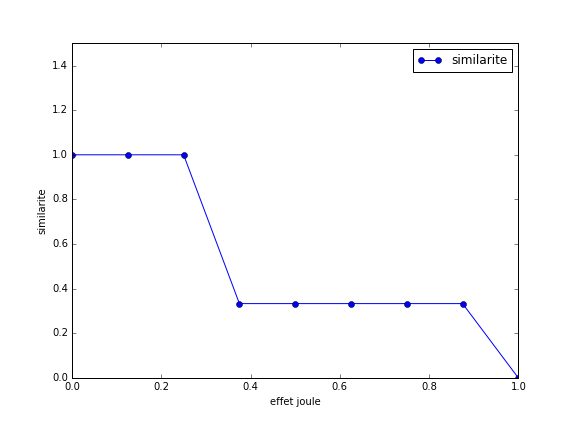
\includegraphics[scale=0.50]{courbe_similarite_selon_EJ_pour_epsilon_075.png}
\caption{ Le coefficient de similarit\'e en fonction des pertes par {\em effets joules} pour $epsilon=0.75$.}
\label {courbeEJCoef}
\end{figure}
\begin{figure}
\centering
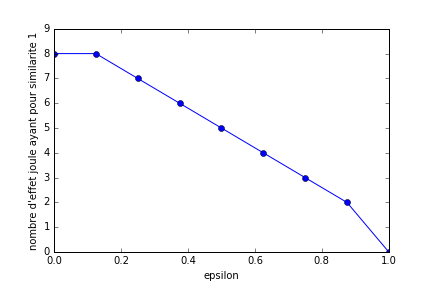
\includegraphics[scale=0.65]{courbe_epsilon_selon_nbreEJ_pour_similarite_1.png}
\caption{ R\'elation inverse entre $\epsilon$ et $EJ$: $8$ en ordonn\'e correspond \`a $[0,1]$, $7$ \`a $[0, 0.875]$ }
\label {courbeEpsilonEJ}
\end{figure}

% conclusion
Ces deux exp\'eriences montrent que la d\'ecision de l'ORACLE  a une r\'elation inverse avec les pertes par effets joules ($EJ$). En effet, plus $\epsilon$ est petit plus les pertes par effets joules sont grandes et plus les d\'ecisions de l'ORACLE sont erron\'ees.
\begin{equation}
	\epsilon > 1 - EJ
\end{equation}

\subsubsection{Complexit\'e de l'algorithme de couverture}
La complexit\'e de l'algorithme est au pire en $O(m \times \Delta(G_M))$ avec $m$ le nombre d'ar\^etes et $\Delta(G_M)$ le degr\'e maximum du graphe.
On rappelle que l'algorithme de Lehot \cite{decompositionEnCliques} a une complexit\'e en $O(m) +E$. 
Le facteur $\Delta(G_M)$ dans notre algorithme, du \`a la recherche de la d\'ecomposition en deux cliques $C_1$ et $C_2$ est n\'ecessaire \`a la determination de l'ensemble des sommets $v$ tels que $Cliq(v) = -1$, en nombre le plus petit possible.
\newline

En conclusion, si le graphe $G_M$ est bien un line-graphe, l'algorithme  de couverture trouvera une d\'ecomposition du voisinage d'un sommet en une ou deux cliques de fa\c con unique (voir les lemmes pr\'ec\'edents). 
Une fois ce sommet supprim\'e, le graphe restant est toujours un line-graphe, et la propri\'et\'e se propage.
Donc, si $G_M$ est un line graphe, cet algorithme en trouvera toujours la couverture de corr\'elation unique.
